\documentclass[11pt,a4paper]{article}
\usepackage[utf8]{inputenc}
\usepackage[left=2.3cm,right=2.3cm,top=2.5cm,bottom=2.5cm]{geometry}
\usepackage{amsmath,amssymb,amsfonts}
\usepackage{array}
\usepackage{enumitem}
\usepackage{fancyhdr}
\setlength{\headheight}{14pt}
\usepackage{hyperref}
\usepackage{tikz}
\usetikzlibrary{arrows.meta, positioning, calc, shapes.geometric}

\tikzset{
    sfgnode/.style={circle, fill=blue!15, draw=blue!70, thick, minimum size=7mm, inner sep=0pt, font=\small\bfseries},
    sfgterminal/.style={circle, fill=gray!15, draw=gray!70, thick, minimum size=7mm, inner sep=0pt, font=\small\bfseries},
    sfgarrow/.style={-{Latex[length=2.5mm,width=1.5mm]}, thick, draw=blue!80!black},
    sfgloop/.style={-{Latex[length=2.5mm,width=1.5mm]}, thick, draw=red!75!black},
    sfgbypass/.style={-{Latex[length=2.5mm,width=1.5mm]}, thick, draw=teal!80!black}
}

\pagestyle{fancy}
\fancyhf{}
\rhead{\textbf{MA4171 Teori Kontrol Linear}}
\lhead{\textbf{Latihan 02: Pemodelan Sistem Dinamik}}
\rfoot{Halaman \thepage}

\hypersetup{
    colorlinks=true,
    linkcolor=blue,
    urlcolor=cyan
}

\setlength{\parindent}{0pt}
\setlength{\parskip}{5pt}

\begin{document}

\begin{center}
    {\Large \textbf{LEMBAR LATIHAN DAN PEMBAHASAN LENGKAP}}\\[4pt]
    {\large \textbf{TOPIK 02: PEMODELAN SISTEM DINAMIK}}\\[4pt]
    \textbf{Mata Kuliah:} MA4171 Teori Kontrol Linear
\end{center}
\hrule
\vspace{10pt}

% =========================================================================
% SOAL 1
% =========================================================================
\textbf{\large No. 1}

\textbf{Soal:}  
Suatu sistem mekanik translasi terdiri dari dua massa $m_1$ dan $m_2$ yang berada di atas lantai licin tanpa gesekan. Massa $m_1$ digerakkan oleh gaya luar $u(t)$ dan dihubungkan ke dinding diam di sebelah kiri melalui pegas $k_1$ dan peredam viskos $b_1$. Di antara massa $m_1$ dan $m_2$, terpasang pegas kedua $k_2$ dan peredam kedua $b_2$. Posisi perpindahan translasi massa $m_1$ dinyatakan sebagai $y_1(t)$ dan massa $m_2$ sebagai $y_2(t)$, keduanya diukur ke arah kanan dari posisi kesetimbangan masing-masing.
\begin{enumerate}[label=(\alph*)]
    \item Turunkan sistem persamaan diferensial gerak kedua massa.
    \item Tentukan representasi ruang keadaan matriks standar $(A, B, C, D)$ dengan vektor keadaan $\mathbf{x}(t) = [y_1, \dot{y}_1, y_2, \dot{y}_2]^T$ dan vektor keluaran $\mathbf{y}(t) = [y_1, y_2]^T$.
    \item Jika $m_1 = 1\text{ kg}$, $m_2 = 1\text{ kg}$, $k_1 = 3\text{ N/m}$, $k_2 = 2\text{ N/m}$, $b_1 = 2\text{ N}\cdot\text{s/m}$, dan $b_2 = 1\text{ N}\cdot\text{s/m}$, tentukan fungsi alih $G_1(s) = \frac{Y_1(s)}{U(s)}$ dan $G_2(s) = \frac{Y_2(s)}{U(s)}$.
\end{enumerate}

\textbf{Penyelesaian:}

\textbf{(a) Penurunan Persamaan Diferensial Gerak}

Ditinjau diagram benda bebas untuk masing-masing massa sesuai dengan Hukum II Newton.

Untuk massa pertama ($m_1$), gaya penggerak adalah gaya luar $u(t)$, sedangkan gaya penahan berasal dari pegas $k_1$, peredam $b_1$, pegas penghubung $k_2$, dan peredam penghubung $b_2$:
$$m_1 \ddot{y}_1(t) = u(t) - k_1 y_1(t) - b_1 \dot{y}_1(t) - k_2 [y_1(t) - y_2(t)] - b_2 [\dot{y}_1(t) - \dot{y}_2(t)]$$
Penyusunan ulang suku-suku menghasilkan:
$$m_1 \ddot{y}_1(t) + (b_1 + b_2) \dot{y}_1(t) - b_2 \dot{y}_2(t) + (k_1 + k_2) y_1(t) - k_2 y_2(t) = u(t)$$

Untuk massa kedua ($m_2$), gaya yang bekerja sepenuhnya berasal dari interaksi elemen penghubung dengan massa pertama:
$$m_2 \ddot{y}_2(t) = k_2 [y_1(t) - y_2(t)] + b_2 [\dot{y}_1(t) - \dot{y}_2(t)]$$
Pengelompokan suku-suku menghasilkan:
$$m_2 \ddot{y}_2(t) - b_2 \dot{y}_1(t) + b_2 \dot{y}_2(t) - k_2 y_1(t) + k_2 y_2(t) = 0$$

\textbf{(b) Pembentukan Model Ruang Keadaan}

Dengan memilih variabel keadaan $x_1 = y_1, x_2 = \dot{y}_1, x_3 = y_2, x_4 = \dot{y}_2$, turunan pertama masing-masing variabel keadaan adalah:
$$\dot{x}_1 = x_2, \quad \dot{x}_2 = -\frac{k_1 + k_2}{m_1} x_1 - \frac{b_1 + b_2}{m_1} x_2 + \frac{k_2}{m_1} x_3 + \frac{b_2}{m_1} x_4 + \frac{1}{m_1} u$$
$$\dot{x}_3 = x_4, \quad \dot{x}_4 = \frac{k_2}{m_2} x_1 + \frac{b_2}{m_2} x_2 - \frac{k_2}{m_2} x_3 - \frac{b_2}{m_2} x_4$$

Dalam bentuk matriks $\dot{\mathbf{x}} = A\mathbf{x} + B u$ dan $\mathbf{y} = C\mathbf{x} + D u$:
$$A = \begin{bmatrix} 0 & 1 & 0 & 0 \\ -\frac{k_1 + k_2}{m_1} & -\frac{b_1 + b_2}{m_1} & \frac{k_2}{m_1} & \frac{b_2}{m_1} \\ 0 & 0 & 0 & 1 \\ \frac{k_2}{m_2} & \frac{b_2}{m_2} & -\frac{k_2}{m_2} & -\frac{b_2}{m_2} \end{bmatrix}, \quad B = \begin{bmatrix} 0 \\ \frac{1}{m_1} \\ 0 \\ 0 \end{bmatrix}, \quad C = \begin{bmatrix} 1 & 0 & 0 & 0 \\ 0 & 0 & 1 & 0 \end{bmatrix}, \quad D = \begin{bmatrix} 0 \\ 0 \end{bmatrix}$$

\textbf{(c) Penentuan Fungsi Alih}

Melalui Transformasi Laplace persamaan gerak dengan kondisi awal nol dan substitusi nilai numerik:
$$(s^2 + 3s + 5) Y_1(s) - (s + 2) Y_2(s) = U(s)$$
$$-(s + 2) Y_1(s) + (s^2 + s + 2) Y_2(s) = 0 \implies Y_2(s) = \frac{s + 2}{s^2 + s + 2} Y_1(s)$$

Substitusi $Y_2(s)$ ke persamaan pertama menghasilkan:
$$\left[ (s^2 + 3s + 5) - \frac{(s+2)^2}{s^2 + s + 2} \right] Y_1(s) = U(s)$$
$$\frac{s^4 + 4s^3 + 9s^2 + 7s + 6}{s^2 + s + 2} Y_1(s) = U(s)$$

Sehingga diperoleh fungsi alih masing-masing keluaran:
$$G_1(s) = \frac{Y_1(s)}{U(s)} = \frac{s^2 + s + 2}{s^4 + 4s^3 + 9s^2 + 7s + 6}$$
$$G_2(s) = \frac{Y_2(s)}{U(s)} = \frac{s + 2}{s^4 + 4s^3 + 9s^2 + 7s + 6}$$

\vspace{12pt}
\hrule
\vspace{10pt}

% =========================================================================
% SOAL 2
% =========================================================================
\textbf{\large No. 2}

\textbf{Soal:}  
Suatu rangkaian listrik terdiri dari sumber tegangan masukan $u(t) = v_{in}(t)$, resistor $R_1$, induktor $L$, kapasitor $C_1$, resistor $R_2$, dan kapasitor $C_2$. Arus pada induktor dinotasikan sebagai $i_L(t)$, tegangan pada kapasitor pertama sebagai $v_{C1}(t)$, dan tegangan pada kapasitor kedua sebagai $v_{C2}(t)$ yang sekaligus menjadi tegangan keluaran $y(t) = v_{C2}(t)$. Rangkaian tersusun dalam bentuk tangga (\textit{ladder network}) di mana masukan terhubung seri dengan $R_1$ dan $L$ menuju simpul kapasitor $C_1$ (terhubung paralel ke ground), yang kemudian dihubungkan melalui $R_2$ ke kapasitor $C_2$ (paralel ke ground).
\begin{enumerate}[label=(\alph*)]
    \item Terapkan Hukum Tegangan Kirchhoff (KVL) dan Hukum Arus Kirchhoff (KCL) untuk menurunkan persamaan dinamik rangkaian.
    \item Susun representasi ruang keadaan dengan vektor keadaan $\mathbf{x}(t) = [i_L(t), v_{C1}(t), v_{C2}(t)]^T$.
    \item Tentukan fungsi alih sistem $G(s) = \frac{V_{C2}(s)}{V_{in}(s)}$ dalam bentuk parameter umum.
\end{enumerate}

\textbf{Penyelesaian:}

\textbf{(a) Penerapan KVL dan KCL}

KVL diterapkan pada loop masukan yang memuat sumber tegangan, resistor $R_1$, induktor $L$, dan kapasitor $C_1$:
$$v_{in}(t) - R_1 i_L(t) - L \frac{di_L(t)}{dt} - v_{C1}(t) = 0$$
$$\implies \frac{di_L}{dt} = -\frac{R_1}{L} i_L - \frac{1}{L} v_{C1} + \frac{1}{L} v_{in}$$

KCL diterapkan pada simpul tegangan $v_{C1}$, di mana arus induktor $i_L$ terbagi menjadi arus yang melewati kapasitor $C_1$ dan arus yang mengalir melalui resistor $R_2$ menuju kapasitor $C_2$:
$$i_L(t) = C_1 \frac{dv_{C1}(t)}{dt} + \frac{v_{C1}(t) - v_{C2}(t)}{R_2}$$
$$\implies \frac{dv_{C1}}{dt} = \frac{1}{C_1} i_L - \frac{1}{R_2 C_1} v_{C1} + \frac{1}{R_2 C_1} v_{C2}$$

KCL diterapkan pada simpul tegangan $v_{C2}$, di mana arus dari resistor $R_2$ seluruhnya mengisi kapasitor $C_2$:
$$\frac{v_{C1}(t) - v_{C2}(t)}{R_2} = C_2 \frac{dv_{C2}(t)}{dt}$$
$$\implies \frac{dv_{C2}}{dt} = \frac{1}{R_2 C_2} v_{C1} - \frac{1}{R_2 C_2} v_{C2}$$

\textbf{(b) Formulasi Model Ruang Keadaan}

Dengan mendefinisikan $x_1 = i_L$, $x_2 = v_{C1}$, dan $x_3 = v_{C2}$, sistem persamaan diferensial di atas dituliskan dalam bentuk matriks:
$$\begin{bmatrix} \dot{x}_1 \\ \dot{x}_2 \\ \dot{x}_3 \end{bmatrix} = \begin{bmatrix} -\frac{R_1}{L} & -\frac{1}{L} & 0 \\ \frac{1}{C_1} & -\frac{1}{R_2 C_1} & \frac{1}{R_2 C_1} \\ 0 & \frac{1}{R_2 C_2} & -\frac{1}{R_2 C_2} \end{bmatrix} \begin{bmatrix} x_1 \\ x_2 \\ x_3 \end{bmatrix} + \begin{bmatrix} \frac{1}{L} \\ 0 \\ 0 \end{bmatrix} u(t)$$

Persamaan keluaran untuk tegangan $y(t) = v_{C2}(t) = x_3(t)$ adalah:
$$y(t) = \begin{bmatrix} 0 & 0 & 1 \end{bmatrix} \begin{bmatrix} x_1 \\ x_2 \\ x_3 \end{bmatrix} + [0] u(t)$$

\textbf{(c) Penentuan Fungsi Alih Sistem}

Dalam domain Laplace dengan kondisi awal nol, persamaan simpul kedua menyatakan hubungan $V_{C1}(s)$ dan $V_{C2}(s)$:
$$V_{C1}(s) = (R_2 C_2 s + 1) V_{C2}(s)$$

Substitusi hubungan ini ke persamaan simpul pertama menghasilkan arus induktor:
\begin{align*}
    I_L(s) &= \left[ C_1 s + \frac{1}{R_2} \right] V_{C1}(s) - \frac{1}{R_2} V_{C2}(s) \\
    &= \left[ C_1 s(R_2 C_2 s + 1) + C_2 s \right] V_{C2}(s) \\
    &= \left[ R_2 C_1 C_2 s^2 + (C_1 + C_2) s \right] V_{C2}(s)
\end{align*}

Substitusi $I_L(s)$ dan $V_{C1}(s)$ ke dalam persamaan KVL loop masukan $(L s + R_1) I_L(s) + V_{C1}(s) = V_{in}(s)$ menghasilkan:
$$\left\{ (L s + R_1)\left[ R_2 C_1 C_2 s^2 + (C_1 + C_2) s \right] + (R_2 C_2 s + 1) \right\} V_{C2}(s) = V_{in}(s)$$

Penguraian polinomial penyebut memberikan fungsi alih:
$$G(s) = \frac{V_{C2}(s)}{V_{in}(s)} = \frac{1}{L R_2 C_1 C_2 s^3 + [L(C_1 + C_2) + R_1 R_2 C_1 C_2] s^2 + [R_1(C_1 + C_2) + R_2 C_2] s + 1}$$

\vspace{12pt}
\hrule
\vspace{10pt}

% =========================================================================
% SOAL 3
% =========================================================================
\textbf{\large No. 3}

\textbf{Soal:}  
Suatu motor arus searah terkendali jangkar (\textit{armature-controlled DC motor}) memiliki resistansi armatur $R_a$, induktansi armatur $L_a$, konstanta torsi $K_t$, konstanta gaya gerak listrik balik (\textit{back-emf}) $K_b$, momen inersia rotor $J$, dan koefisien gesekan redaman viskos $B_m$. Masukan sistem adalah tegangan armatur $u(t) = v_a(t)$, sedangkan keluaran yang diamati adalah posisi sudut rotor $y_1(t) = \theta(t)$ dan kecepatan sudut rotor $y_2(t) = \omega(t) = \dot{\theta}(t)$.
\begin{enumerate}[label=(\alph*)]
    \item Turunkan persamaan diferensial yang mengatur dinamika elektrik dan mekanik motor.
    \item Susun model ruang keadaan dengan vektor keadaan $\mathbf{x}(t) = [\theta(t), \omega(t), i_a(t)]^T$.
    \item Diberikan nilai parameter: $R_a = 2\,\Omega$, $L_a = 0.5\text{ H}$, $K_t = 0.1\text{ N}\cdot\text{m/A}$, $K_b = 0.1\text{ V}\cdot\text{s/rad}$, $J = 0.02\text{ kg}\cdot\text{m}^2$, dan $B_m = 0.01\text{ N}\cdot\text{m}\cdot\text{s/rad}$. Tentukan fungsi alih posisi $G_\theta(s) = \frac{\Theta(s)}{V_a(s)}$ dan fungsi alih kecepatan $G_\omega(s) = \frac{\Omega(s)}{V_a(s)}$.
\end{enumerate}

\textbf{Penyelesaian:}

\textbf{(a) Penurunan Persamaan Dinamika Elektromekanik}

Sirkuit elektrik armatur memenuhi persamaan tegangan KVL dengan tegangan balik $e_b(t) = K_b \omega(t)$:
$$L_a \frac{di_a(t)}{dt} + R_a i_a(t) + K_b \omega(t) = v_a(t) \implies \frac{di_a}{dt} = -\frac{R_a}{L_a} i_a - \frac{K_b}{L_a} \omega + \frac{1}{L_a} v_a$$

Dinamika mekanik rotor memenuhi Hukum II Newton untuk gerak rotasi dengan torsi elektromagnetik $T_m(t) = K_t i_a(t)$:
$$J \frac{d\omega(t)}{dt} + B_m \omega(t) = K_t i_a(t) \implies \frac{d\omega}{dt} = -\frac{B_m}{J} \omega + \frac{K_t}{J} i_a$$

Hubungan antara posisi sudut dan kecepatan sudut rotor adalah $\frac{d\theta}{dt} = \omega(t)$.

\textbf{(b) Formulasi Model Ruang Keadaan}

Dengan variabel keadaan $x_1 = \theta, x_2 = \omega, x_3 = i_a$, matriks ruang keadaan dinyatakan sebagai:
$$\begin{bmatrix} \dot{x}_1 \\ \dot{x}_2 \\ \dot{x}_3 \end{bmatrix} = \begin{bmatrix} 0 & 1 & 0 \\ 0 & -\frac{B_m}{J} & \frac{K_t}{J} \\ 0 & -\frac{K_b}{L_a} & -\frac{R_a}{L_a} \end{bmatrix} \begin{bmatrix} x_1 \\ x_2 \\ x_3 \end{bmatrix} + \begin{bmatrix} 0 \\ 0 \\ \frac{1}{L_a} \end{bmatrix} u(t)$$

Persamaan keluaran untuk posisi dan kecepatan sudut rotor adalah:
$$\mathbf{y}(t) = \begin{bmatrix} 1 & 0 & 0 \\ 0 & 1 & 0 \end{bmatrix} \begin{bmatrix} x_1 \\ x_2 \\ x_3 \end{bmatrix} + \begin{bmatrix} 0 \\ 0 \end{bmatrix} u(t)$$

\textbf{(c) Penentuan Fungsi Alih Numerik}

Dalam domain Laplace dengan kondisi awal nol, persamaan elektrik dan mekanik menghasilkan:
$$I_a(s) = \frac{V_a(s) - K_b \Omega(s)}{L_a s + R_a}$$
$$(J s + B_m) \Omega(s) = K_t I_a(s) = K_t \left[ \frac{V_a(s) - K_b \Omega(s)}{L_a s + R_a} \right]$$

Pengelompokan suku $\Omega(s)$ menghasilkan fungsi alih kecepatan sudut:
$$G_\omega(s) = \frac{\Omega(s)}{V_a(s)} = \frac{K_t}{(J s + B_m)(L_a s + R_a) + K_t K_b} = \frac{K_t}{J L_a s^2 + (J R_a + B_m L_a) s + (B_m R_a + K_t K_b)}$$

Substitusi nilai parameter:
$$J L_a = (0.02)(0.5) = 0.01, \quad J R_a + B_m L_a = (0.02)(2) + (0.01)(0.5) = 0.045$$
$$B_m R_a + K_t K_b = (0.01)(2) + (0.1)(0.1) = 0.02 + 0.01 = 0.03, \quad K_t = 0.1$$

Sehingga diperoleh fungsi alih kecepatan:
$$G_\omega(s) = \frac{0.1}{0.01 s^2 + 0.045 s + 0.03} = \frac{10}{s^2 + 4.5 s + 3}$$

Fungsi alih posisi sudut $\Theta(s) = \frac{1}{s}\Omega(s)$ adalah:
$$G_\theta(s) = \frac{\Theta(s)}{V_a(s)} = \frac{10}{s(s^2 + 4.5 s + 3)} = \frac{10}{s^3 + 4.5 s^2 + 3s}$$

\vspace{12pt}
\hrule
\vspace{10pt}

% =========================================================================
% SOAL 4
% =========================================================================
\textbf{\large No. 4}

\textbf{Soal:}  
Suatu sistem tangki bertingkat terhubung (\textit{interacting two-tank system}) memiliki dua tangki penampung cairan dengan luas penampang seragam $A_1$ dan $A_2$. Cairan masuk ke tangki 1 dengan laju volumetrik $u(t) = q_{in}(t)$. Cairan mengalir dari tangki 1 ke tangki 2 melalui pipa berhambatan hidrolik $R_1$ dengan debit $q_1(t) = \frac{h_1(t) - h_2(t)}{R_1}$, dan mengalir keluar dari tangki 2 ke udara bebas melalui pipa berhambatan $R_2$ dengan debit $q_2(t) = \frac{h_2(t)}{R_2}$. Variabel tinggi permukaan cairan pada masing-masing tangki adalah $h_1(t)$ dan $h_2(t)$, dengan keluaran sistem adalah $y(t) = h_2(t)$.
\begin{enumerate}[label=(\alph*)]
    \item Turunkan persamaan diferensial neraca massa laju aliran untuk kedua tangki.
    \item Susun representasi ruang keadaan matriks dengan vektor keadaan $\mathbf{x}(t) = [h_1(t), h_2(t)]^T$.
    \item Tentukan fungsi alih loop terbuka $G(s) = \frac{H_2(s)}{Q_{in}(s)}$.
\end{enumerate}

\textbf{Penyelesaian:}

\textbf{(a) Penurunan Persamaan Neraca Massa}

Neraca massa cairan pada tangki 1 menyatakan bahwa laju akumulasi volume cairan sama dengan selisih debit masuk dan debit keluar:
$$A_1 \frac{dh_1(t)}{dt} = q_{in}(t) - q_1(t) = u(t) - \frac{h_1(t) - h_2(t)}{R_1}$$
$$\implies \frac{dh_1}{dt} = -\frac{1}{A_1 R_1} h_1 + \frac{1}{A_1 R_1} h_2 + \frac{1}{A_1} u$$

Neraca massa cairan pada tangki 2 menyatakan bahwa laju akumulasi volume cairan sama dengan debit masuk dari tangki 1 dikurangi debit keluar tangki 2:
$$A_2 \frac{dh_2(t)}{dt} = q_1(t) - q_2(t) = \frac{h_1(t) - h_2(t)}{R_1} - \frac{h_2(t)}{R_2}$$
$$\implies \frac{dh_2}{dt} = \frac{1}{A_2 R_1} h_1 - \left( \frac{1}{A_2 R_1} + \frac{1}{A_2 R_2} \right) h_2$$

\textbf{(b) Formulasi Model Ruang Keadaan}

Dengan vektor keadaan $\mathbf{x} = [h_1, h_2]^T$ dan masukan $u = q_{in}$, persamaan ruang keadaan matriks adalah:
$$\begin{bmatrix} \dot{h}_1 \\ \dot{h}_2 \end{bmatrix} = \begin{bmatrix} -\frac{1}{A_1 R_1} & \frac{1}{A_1 R_1} \\ \frac{1}{A_2 R_1} & -\left(\frac{1}{A_2 R_1} + \frac{1}{A_2 R_2}\right) \end{bmatrix} \begin{bmatrix} h_1 \\ h_2 \end{bmatrix} + \begin{bmatrix} \frac{1}{A_1} \\ 0 \end{bmatrix} u(t)$$

Persamaan keluaran untuk ketinggian cairan pada tangki kedua adalah:
$$y(t) = \begin{bmatrix} 0 & 1 \end{bmatrix} \begin{bmatrix} h_1 \\ h_2 \end{bmatrix} + [0] u(t)$$

\textbf{(c) Penentuan Fungsi Alih Sistem}

Dengan melakukan Transformasi Laplace pada kedua persamaan neraca massa dengan kondisi awal nol:
$$(A_1 R_1 s + 1) H_1(s) - H_2(s) = R_1 Q_{in}(s) \implies H_1(s) = \frac{R_1 Q_{in}(s) + H_2(s)}{A_1 R_1 s + 1}$$
$$-H_1(s) + \left( \frac{R_1}{R_2} + A_2 R_1 s + 1 \right) H_2(s) = 0 \implies H_1(s) = \left( A_2 R_1 s + 1 + \frac{R_1}{R_2} \right) H_2(s)$$

Penyamaan kedua ekspresi $H_1(s)$ menghasilkan:
$$\left[ (A_1 R_1 s + 1)\left( A_2 R_1 s + 1 + \frac{R_1}{R_2} \right) - 1 \right] H_2(s) = R_1 Q_{in}(s)$$

Penguraian kurung siku menghasilkan:
\begin{align*}
    &\left[ A_1 A_2 R_1^2 s^2 + \left( A_1 R_1\left(1 + \frac{R_1}{R_2}\right) + A_2 R_1 \right) s + \frac{R_1}{R_2} \right] H_2(s) = R_1 Q_{in}(s) \\
    &\implies \frac{R_1}{R_2} \left[ A_1 A_2 R_1 R_2 s^2 + (A_1 R_1 + A_1 R_2 + A_2 R_2) s + 1 \right] H_2(s) = R_1 Q_{in}(s)
\end{align*}

Dengan membagi kedua ruas dengan $R_1$, diperoleh fungsi alih:
$$G(s) = \frac{H_2(s)}{Q_{in}(s)} = \frac{R_2}{A_1 A_2 R_1 R_2 s^2 + (A_1 R_1 + A_1 R_2 + A_2 R_2) s + 1}$$

\vspace{12pt}
\hrule
\vspace{10pt}

% =========================================================================
% SOAL 5
% =========================================================================
\textbf{\large No. 5}

\textbf{Soal:}  
Suatu sistem kendali loop tertutup dengan konfigurasi umpan balik ganda memiliki hubungan blok sebagai berikut: sinyal masukan $R(s)$ masuk ke titik penjumlahan 1 (+) bersama umpan balik negatif $-H_2(s) Y(s)$ menghasilkan sinyal $E_1(s)$. Sinyal $E_1(s)$ melewati blok $G_1(s)$ menuju titik penjumlahan 2 (+), yang juga menerima umpan balik negatif $-H_1(s)$ dari keluaran blok $G_2(s)$. Keluaran titik penjumlahan 2 masuk ke blok $G_2(s)$, menghasilkan sinyal $V(s)$. Sinyal $V(s)$ dijumlahkan di titik penjumlahan 3 (+) dengan sinyal \textit{feedforward} $+G_3(s) E_1(s)$, dan hasilnya melewati blok $G_4(s)$ untuk menghasilkan keluaran akhir $Y(s)$.
\begin{enumerate}[label=(\alph*)]
    \item Tuliskan persamaan aljabar sinyal pada setiap titik percabangan dan titik penjumlahan.
    \item Lakukan reduksi diagram blok secara analitis untuk menentukan fungsi alih loop tertutup $T(s) = \frac{Y(s)}{R(s)}$.
\end{enumerate}

\textbf{Penyelesaian:}

\textbf{(a) Persamaan Aljabar Diagram Blok}

Persamaan sinyal pada masing-masing titik diagram blok adalah:
$$E_1(s) = R(s) - H_2(s) Y(s)$$
$$V(s) = G_2(s) \left[ G_1(s) E_1(s) - H_1(s) V(s) \right]$$
$$Y(s) = G_4(s) \left[ V(s) + G_3(s) E_1(s) \right]$$

\textbf{(b) Reduksi Aljabar Fungsi Alih}

Penyelesaian persamaan internal untuk sinyal $V(s)$ dalam fungsi $E_1(s)$ menghasilkan:
$$[1 + G_2(s) H_1(s)] V(s) = G_1(s) G_2(s) E_1(s) \implies V(s) = \frac{G_1(s) G_2(s)}{1 + G_2(s) H_1(s)} E_1(s)$$

Substitusi $V(s)$ ke persamaan sinyal keluaran $Y(s)$ menghasilkan:
\begin{align*}
    Y(s) &= G_4(s) \left[ \frac{G_1(s) G_2(s)}{1 + G_2(s) H_1(s)} + G_3(s) \right] E_1(s) \\
    &= G_4(s) \left[ \frac{G_1(s) G_2(s) + G_3(s)(1 + G_2(s) H_1(s))}{1 + G_2(s) H_1(s)} \right] E_1(s)
\end{align*}

Substitusi ekspresi $E_1(s) = R(s) - H_2(s) Y(s)$ menghasilkan persamaan relasi masukan-keluaran:
$$Y(s) = \frac{G_4(s) [G_1(s) G_2(s) + G_3(s) + G_2(s) G_3(s) H_1(s)]}{1 + G_2(s) H_1(s)} [R(s) - H_2(s) Y(s)]$$

Pengelompokan suku $Y(s)$ ke ruas kiri menghasilkan fungsi alih loop tertutup:
$$T(s) = \frac{Y(s)}{R(s)} = \frac{G_1(s) G_2(s) G_4(s) + G_3(s) G_4(s) + G_2(s) G_3(s) G_4(s) H_1(s)}{1 + G_2(s) H_1(s) + H_2(s) G_4(s) [G_1(s) G_2(s) + G_3(s) + G_2(s) G_3(s) H_1(s)]}$$

\vspace{12pt}
\hrule
\vspace{10pt}

% =========================================================================
% SOAL 6
% =========================================================================
\textbf{\large No. 6}

\textbf{Soal:}  
Diberikan diagram aliran sinyal (\textit{Signal Flow Graph} / SFG) dengan simpul masukan $R(s) = x_0$, simpul internal $x_1, x_2, x_3, x_4$, dan simpul keluaran $Y(s) = x_5$. Transmisi antar-simpul diberikan oleh hubungan berikut:
$$x_1 = R - H_1 x_2 - H_3 x_5, \quad x_2 = G_1 x_1 - H_2 x_4, \quad x_3 = G_2 x_2, \quad x_4 = G_3 x_3, \quad x_5 = G_4 x_4 + G_5 x_2$$

\begin{center}
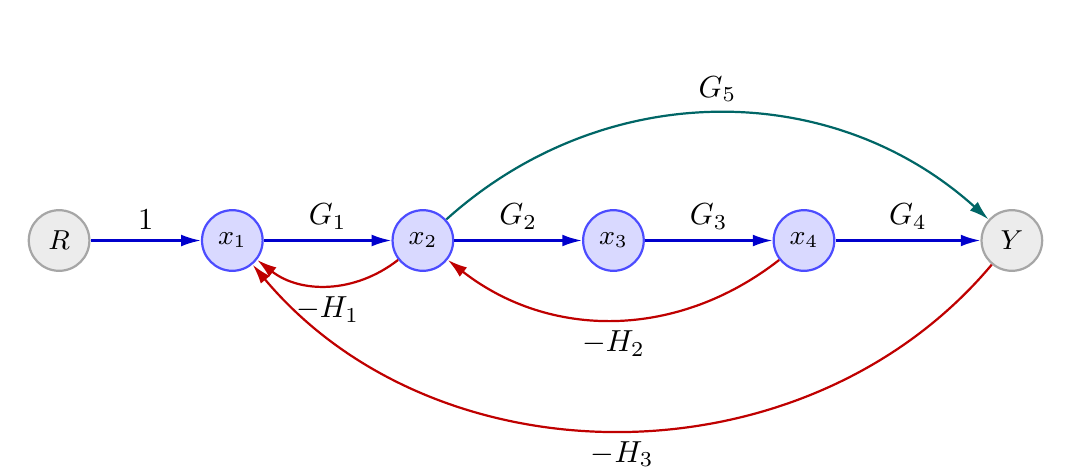
\begin{tikzpicture}[scale=1.1, transform shape]
    \node[sfgterminal] (R) at (0,0) {$R$};
    \node[sfgnode] (x1) at (2,0) {$x_1$};
    \node[sfgnode] (x2) at (4.2,0) {$x_2$};
    \node[sfgnode] (x3) at (6.4,0) {$x_3$};
    \node[sfgnode] (x4) at (8.6,0) {$x_4$};
    \node[sfgterminal] (x5) at (11,0) {$Y$};
    
    % Forward branches
    \draw[sfgarrow] (R) -- node[above] {$1$} (x1);
    \draw[sfgarrow] (x1) -- node[above] {$G_1$} (x2);
    \draw[sfgarrow] (x2) -- node[above] {$G_2$} (x3);
    \draw[sfgarrow] (x3) -- node[above] {$G_3$} (x4);
    \draw[sfgarrow] (x4) -- node[above] {$G_4$} (x5);
    
    % Feedforward bypass
    \draw[sfgbypass] (x2) to[bend left=42] node[above] {$G_5$} (x5);
    
    % Feedback loops
    \draw[sfgloop] (x2) to[bend left=38] node[below] {$-H_1$} (x1);
    \draw[sfgloop] (x4) to[bend left=38] node[below] {$-H_2$} (x2);
    \draw[sfgloop] (x5) to[bend left=50] node[below] {$-H_3$} (x1);
\end{tikzpicture}
\end{center}

\begin{enumerate}[label=(\alph*)]
    \item Tentukan semua lintasan maju (\textit{forward paths}) beserta penguatannya ($F_k$).
    \item Tentukan semua loop umpan balik tunggal ($L_i$) dan pasangan loop tak bersentuhan (\textit{non-touching loops}).
    \item Hitung determinan graf $\Delta$ dan kofaktor lintasan $\Delta_k$.
    \item Tentukan fungsi alih total $G(s) = \frac{Y(s)}{R(s)}$ menggunakan Rumus Penguatan Mason.
\end{enumerate}

\textbf{Penyelesaian:}

\textbf{(a) Penentuan Lintasan Maju ($F_k$)}

Dari simpul masukan $R$ ke simpul keluaran $Y = x_5$, terdapat dua lintasan maju:
Lintasan pertama melalui simpul $R \to x_1 \to x_2 \to x_3 \to x_4 \to x_5$ dengan penguatan:
$$F_1 = (1)(G_1)(G_2)(G_3)(G_4) = G_1 G_2 G_3 G_4$$
Lintasan kedua melewati jalur pintas dari simpul $x_2$ langsung ke $x_5$ melalui $R \to x_1 \to x_2 \to x_5$ dengan penguatan:
$$F_2 = (1)(G_1)(G_5) = G_1 G_5$$

\textbf{(b) Penentuan Loop Tunggal dan Pasangan Loop Saling Lepas}

Loop-loop umpan balik tunggal pada graf adalah:
$$L_1 = x_1 \to x_2 \to x_1 = -G_1 H_1$$
$$L_2 = x_2 \to x_3 \to x_4 \to x_2 = -G_2 G_3 H_2$$
$$L_3 = x_1 \to x_2 \to x_3 \to x_4 \to x_5 \to x_1 = -G_1 G_2 G_3 G_4 H_3$$
$$L_4 = x_1 \to x_2 \to x_5 \to x_1 = -G_1 G_5 H_3$$

Pemeriksaan persinggungan simpul: Loop $L_1$ melibatkan simpul $\{x_1, x_2\}$, sedangkan Loop $L_2$ melibatkan simpul $\{x_2, x_3, x_4\}$. Karena keduanya berbagi simpul $x_2$, maka $L_1$ dan $L_2$ bersentuhan. Loop $L_3$ dan $L_4$ melibatkan seluruh simpul $\{x_1, x_2, \dots\}$. Dengan demikian, \textbf{tidak ada pasangan loop yang saling lepas} (semua loop saling bersentuhan).

\textbf{(c) Perhitungan Determinan $\Delta$ dan Kofaktor $\Delta_k$}

Determinan graf dihitung sebagai:
$$\Delta = 1 - \sum L_i = 1 - (L_1 + L_2 + L_3 + L_4) = 1 + G_1 H_1 + G_2 G_3 H_2 + G_1 G_2 G_3 G_4 H_3 + G_1 G_5 H_3$$

Kofaktor lintasan maju dihitung dengan mengeliminasi loop yang menyentuh lintasan:
Lintasan $F_1$ menyentuh semua simpul $\{x_1, x_2, x_3, x_4, x_5\}$, sehingga menyentuh seluruh loop $\implies \Delta_1 = 1$.
Lintasan $F_2$ melalui simpul $\{x_1, x_2, x_5\}$. Loop $L_2$ yang melalui $\{x_2, x_3, x_4\}$ juga menyentuh simpul $x_2$ pada lintasan $F_2$, sehingga semua loop menyentuh lintasan $F_2 \implies \Delta_2 = 1$.

\textbf{(d) Perhitungan Fungsi Alih Total dengan Rumus Mason}

Penerapan Rumus Penguatan Mason $G(s) = \frac{\sum F_k \Delta_k}{\Delta}$ menghasilkan:
$$G(s) = \frac{Y(s)}{R(s)} = \frac{G_1 G_2 G_3 G_4 + G_1 G_5}{1 + G_1 H_1 + G_2 G_3 H_2 + G_1 G_2 G_3 G_4 H_3 + G_1 G_5 H_3}$$

\vspace{12pt}
\hrule
\vspace{10pt}

% =========================================================================
% SOAL 7
% =========================================================================
\textbf{\large No. 7}

\textbf{Soal:}  
Suatu sistem terkopel 2-masukan 2-keluaran (MIMO) memiliki hubungan sinyal internal yang direpresentasikan oleh SFG dengan masukan $U_1, U_2$ dan keluaran $Y_1, Y_2$ sebagai berikut:
$$Y_1 = G_1 [U_1 - H_1 Y_1] + G_{12} Y_2, \quad Y_2 = G_2 [U_2 - H_2 Y_2] + G_{21} Y_1$$

\begin{center}
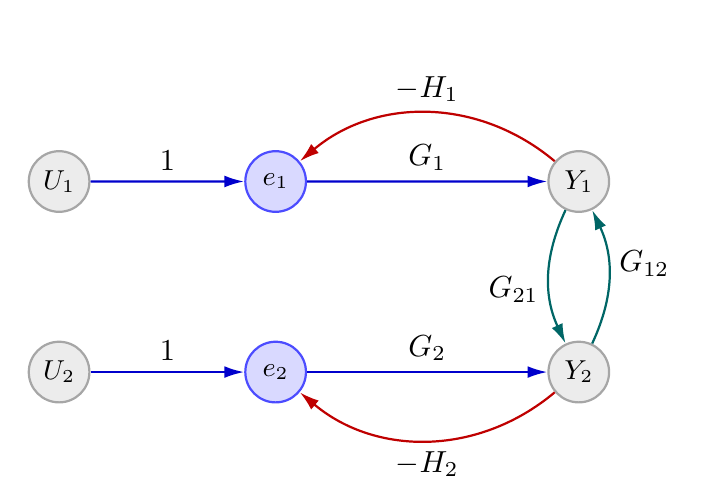
\begin{tikzpicture}[scale=1.1, transform shape]
    \node[sfgterminal] (U1) at (0,2.2) {$U_1$};
    \node[sfgnode] (e1) at (2.5,2.2) {$e_1$};
    \node[sfgterminal] (Y1) at (6,2.2) {$Y_1$};
    
    \node[sfgterminal] (U2) at (0,0) {$U_2$};
    \node[sfgnode] (e2) at (2.5,0) {$e_2$};
    \node[sfgterminal] (Y2) at (6,0) {$Y_2$};
    
    % Forward paths
    \draw[sfgarrow] (U1) -- node[above] {$1$} (e1);
    \draw[sfgarrow] (e1) -- node[above] {$G_1$} (Y1);
    \draw[sfgarrow] (U2) -- node[above] {$1$} (e2);
    \draw[sfgarrow] (e2) -- node[above] {$G_2$} (Y2);
    
    % Local feedbacks
    \draw[sfgloop] (Y1) to[bend right=40] node[above] {$-H_1$} (e1);
    \draw[sfgloop] (Y2) to[bend left=40] node[below] {$-H_2$} (e2);
    
    % Cross-coupling
    \draw[sfgbypass] (Y2) to[bend right=25] node[pos=0.6, right] {$G_{12}$} (Y1);
    \draw[sfgbypass] (Y1) to[bend right=25] node[pos=0.6, left] {$G_{21}$} (Y2);
\end{tikzpicture}
\end{center}

Tentukan matriks fungsi alih transfer sistem $\mathbf{G}_{MIMO}(s) = \begin{bmatrix} G_{11}(s) & G_{12}(s) \\ G_{21}(s) & G_{22}(s) \end{bmatrix}$ sedemikian sehingga $\begin{bmatrix} Y_1(s) \\ Y_2(s) \end{bmatrix} = \mathbf{G}_{MIMO}(s) \begin{bmatrix} U_1(s) \\ U_2(s) \end{bmatrix}$.

\textbf{Penyelesaian:}

Persamaan sistem dapat dituliskan dalam bentuk relasi simpul:
$$(1 + G_1 H_1) Y_1 - G_{12} Y_2 = G_1 U_1$$
$$-G_{21} Y_1 + (1 + G_2 H_2) Y_2 = G_2 U_2$$

Dalam bentuk representasi matriks aljabar:
$$\begin{bmatrix} 1 + G_1 H_1 & -G_{12} \\ -G_{21} & 1 + G_2 H_2 \end{bmatrix} \begin{bmatrix} Y_1 \\ Y_2 \end{bmatrix} = \begin{bmatrix} G_1 & 0 \\ 0 & G_2 \end{bmatrix} \begin{bmatrix} U_1 \\ U_2 \end{bmatrix}$$

Determinan karakteristik graf sistem terkopel adalah:
$$\Delta = (1 + G_1 H_1)(1 + G_2 H_2) - G_{12} G_{21}$$

Invers matriks koefisien dihitung untuk memperoleh hubungan keluaran:
$$\begin{bmatrix} Y_1 \\ Y_2 \end{bmatrix} = \frac{1}{\Delta} \begin{bmatrix} 1 + G_2 H_2 & G_{12} \\ G_{21} & 1 + G_1 H_1 \end{bmatrix} \begin{bmatrix} G_1 & 0 \\ 0 & G_2 \end{bmatrix} \begin{bmatrix} U_1 \\ U_2 \end{bmatrix}$$

Perkalian matriks menghasilkan elemen-elemen matriks transfer:
$$\mathbf{G}_{MIMO}(s) = \frac{1}{(1 + G_1 H_1)(1 + G_2 H_2) - G_{12} G_{21}} \begin{bmatrix} G_1(1 + G_2 H_2) & G_2 G_{12} \\ G_1 G_{21} & G_2(1 + G_1 H_1) \end{bmatrix}$$

\vspace{12pt}
\hrule
\vspace{10pt}

% =========================================================================
% SOAL 8
% =========================================================================
\textbf{\large No. 8}

\textbf{Soal:}  
Diberikan diagram aliran sinyal yang tersusun atas 3 buah integrator berurutan ($1/s$) dengan variabel keadaan $x_1, x_2, x_3$ didefinisikan sebagai sinyal keluaran dari masing-masing integrator dari kiri ke kanan (masukan integrator masing-masing adalah $\dot{x}_1, \dot{x}_2, \dot{x}_3$). Topologi percabangan sistem didefinisikan sebagai:
$$\dot{x}_1 = -a_1 x_1 + x_2 + b_1 u, \quad \dot{x}_2 = -a_2 x_1 + x_3 + b_2 u, \quad \dot{x}_3 = -a_3 x_1 + b_3 u, \quad y = c_1 x_1 + c_2 x_2 + c_3 x_3 + d u$$

\begin{center}
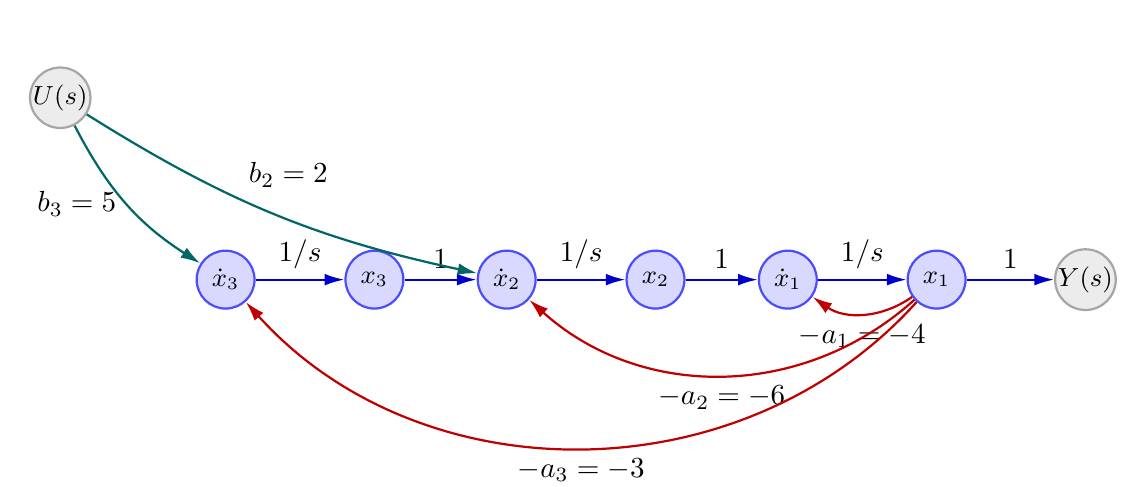
\begin{tikzpicture}[scale=1.05, transform shape]
    \node[sfgterminal] (U) at (0,2.2) {$U(s)$};
    \node[sfgnode] (dx3) at (2,0) {$\dot{x}_3$};
    \node[sfgnode] (x3) at (3.8,0) {$x_3$};
    \node[sfgnode] (dx2) at (5.4,0) {$\dot{x}_2$};
    \node[sfgnode] (x2) at (7.2,0) {$x_2$};
    \node[sfgnode] (dx1) at (8.8,0) {$\dot{x}_1$};
    \node[sfgnode] (x1) at (10.6,0) {$x_1$};
    \node[sfgterminal] (Y) at (12.4,0) {$Y(s)$};
    
    % Integrators
    \draw[sfgarrow] (dx3) -- node[above] {$1/s$} (x3);
    \draw[sfgarrow] (x3) -- node[above] {$1$} (dx2);
    \draw[sfgarrow] (dx2) -- node[above] {$1/s$} (x2);
    \draw[sfgarrow] (x2) -- node[above] {$1$} (dx1);
    \draw[sfgarrow] (dx1) -- node[above] {$1/s$} (x1);
    \draw[sfgarrow] (x1) -- node[above] {$1$} (Y);
    
    % Input injections
    \draw[sfgbypass] (U) to[bend right=15] node[left] {$b_3=5$} (dx3);
    \draw[sfgbypass] (U) to[bend right=10] node[pos=0.4, above right] {$b_2=2$} (dx2);
    
    % Feedbacks from x1
    \draw[sfgloop] (x1) to[bend left=35] node[below] {$-a_1=-4$} (dx1);
    \draw[sfgloop] (x1) to[bend left=42] node[below] {$-a_2=-6$} (dx2);
    \draw[sfgloop] (x1) to[bend left=48] node[below] {$-a_3=-3$} (dx3);
\end{tikzpicture}
\end{center}

Susun matriks ruang keadaan $(A, B, C, D)$ sistem tersebut secara langsung dan tentukan fungsi alih $G(s) = \frac{Y(s)}{U(s)}$ ketika $b_1=0, b_2=2, b_3=5, a_1=4, a_2=6, a_3=3, c_1=1, c_2=0, c_3=0, d=0$.

\textbf{Penyelesaian:}

Dari relasi topologi simpul, matriks dinamik sistem dapat disusun secara langsung:
$$A = \begin{bmatrix} -a_1 & 1 & 0 \\ -a_2 & 0 & 1 \\ -a_3 & 0 & 0 \end{bmatrix}, \quad B = \begin{bmatrix} b_1 \\ b_2 \\ b_3 \end{bmatrix}, \quad C = \begin{bmatrix} c_1 & c_2 & c_3 \end{bmatrix}, \quad D = [d]$$

Struktur ini merupakan bentuk \textit{Observable Canonical Form} (OCF). Untuk nilai-nilai numerik yang diberikan:
$$A = \begin{bmatrix} -4 & 1 & 0 \\ -6 & 0 & 1 \\ -3 & 0 & 0 \end{bmatrix}, \quad B = \begin{bmatrix} 0 \\ 2 \\ 5 \end{bmatrix}, \quad C = \begin{bmatrix} 1 & 0 & 0 \end{bmatrix}, \quad D = [0]$$

Determinan matriks karakteristik dihitung melalui ekspansi minor:
$$\det(sI - A) = \det \begin{bmatrix} s+4 & -1 & 0 \\ 6 & s & -1 \\ 3 & 0 & s \end{bmatrix} = (s+4)(s^2) - (-1)(6s + 3) = s^3 + 4s^2 + 6s + 3$$

Fungsi alih sistem diperoleh melalui perumusan $Y(s) = X_1(s)$:
\begin{align*}
    s X_1(s) &= -4 X_1(s) + X_2(s) \implies X_2(s) = (s+4) X_1(s) \\
    s X_2(s) &= -6 X_1(s) + X_3(s) + 2 U(s) \implies X_3(s) = (s^2 + 4s + 6) X_1(s) - 2 U(s) \\
    s X_3(s) &= -3 X_1(s) + 5 U(s)
\end{align*}

Substitusi $X_3(s)$ ke persamaan terakhir menghasilkan:
$$s [(s^2 + 4s + 6) X_1(s) - 2 U(s)] = -3 X_1(s) + 5 U(s)$$
$$(s^3 + 4s^2 + 6s + 3) X_1(s) = (2s + 5) U(s)$$

Karena $Y(s) = X_1(s)$, maka fungsi alih sistem adalah:
$$G(s) = \frac{Y(s)}{U(s)} = \frac{2s + 5}{s^3 + 4s^2 + 6s + 3}$$

\vspace{12pt}
\hrule
\vspace{10pt}

% =========================================================================
% SOAL 9
% =========================================================================
\textbf{\large No. 9}

\textbf{Soal:}  
Diberikan fungsi alih rasional berderajat 3 bertipe \textit{proper} sebagai berikut:
$$G(s) = \frac{2s^3 + 13s^2 + 24s + 15}{s^3 + 6s^2 + 11s + 6}$$
\begin{enumerate}[label=(\alph*)]
    \item Pisahkan suku transmisi langsung (\textit{direct feedthrough}) $d_0$ dan bentuk fungsi alih menjadi bagian \textit{strictly proper}.
    \item Tentukan representasi ruang keadaan dalam Bentuk Kanonik Terkontrol (\textit{Controllable Canonical Form} - CCF) dan gambarkan diagram aliran sinyalnya.
\end{enumerate}

\textbf{Penyelesaian:}

\textbf{(a) Pemisahan Bagian Strictly Proper}

Pembagian polinomial pembilang oleh penyebut menghasilkan:
$$2s^3 + 13s^2 + 24s + 15 = 2(s^3 + 6s^2 + 11s + 6) + (s^2 + 2s + 3)$$

Dengan demikian fungsi alih dapat dituliskan sebagai:
$$G(s) = d_0 + G_{sp}(s) = 2 + \frac{s^2 + 2s + 3}{s^3 + 6s^2 + 11s + 6}$$
dengan $d_0 = 2$, $b_2 = 1, b_1 = 2, b_0 = 3$, serta koefisien penyebut $a_2 = 6, a_1 = 11, a_0 = 6$.

\textbf{(b) Formulasi Controllable Canonical Form (CCF) \& Diagram SFG}

Berdasarkan definisi standar CCF untuk penyebut $s^3 + a_2 s^2 + a_1 s + a_0$ dan pembilang $b_2 s^2 + b_1 s + b_0$:
$$A_{CCF} = \begin{bmatrix} 0 & 1 & 0 \\ 0 & 0 & 1 \\ -a_0 & -a_1 & -a_2 \end{bmatrix} = \begin{bmatrix} 0 & 1 & 0 \\ 0 & 0 & 1 \\ -6 & -11 & -6 \end{bmatrix}$$
$$B_{CCF} = \begin{bmatrix} 0 \\ 0 \\ 1 \end{bmatrix}, \quad C_{CCF} = \begin{bmatrix} b_0 & b_1 & b_2 \end{bmatrix} = \begin{bmatrix} 3 & 2 & 1 \end{bmatrix}, \quad D_{CCF} = [d_0] = [2]$$

\begin{center}
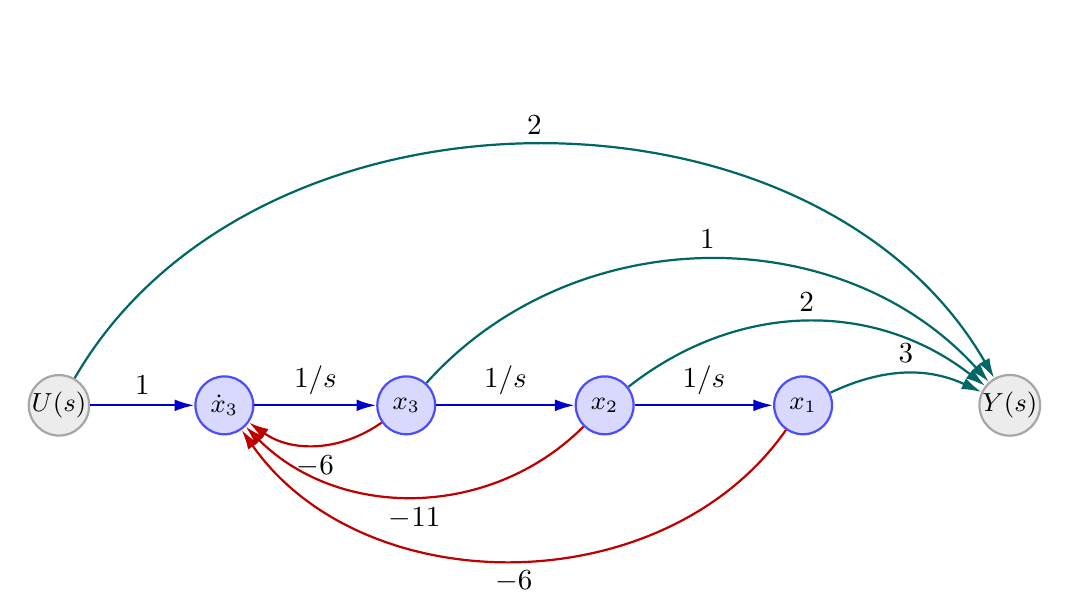
\begin{tikzpicture}[scale=1.05, transform shape]
    \node[sfgterminal] (U) at (0,0) {$U(s)$};
    \node[sfgnode] (dx3) at (2,0) {$\dot{x}_3$};
    \node[sfgnode] (x3) at (4.2,0) {$x_3$};
    \node[sfgnode] (x2) at (6.6,0) {$x_2$};
    \node[sfgnode] (x1) at (9,0) {$x_1$};
    \node[sfgterminal] (Y) at (11.5,0) {$Y(s)$};
    
    % Integrator chain
    \draw[sfgarrow] (U) -- node[above] {$1$} (dx3);
    \draw[sfgarrow] (dx3) -- node[above] {$1/s$} (x3);
    \draw[sfgarrow] (x3) -- node[above] {$1/s$} (x2);
    \draw[sfgarrow] (x2) -- node[above] {$1/s$} (x1);
    
    % Feedbacks to dx3
    \draw[sfgloop] (x3) to[bend left=35] node[below] {$-6$} (dx3);
    \draw[sfgloop] (x2) to[bend left=45] node[below] {$-11$} (dx3);
    \draw[sfgloop] (x1) to[bend left=55] node[below] {$-6$} (dx3);
    
    % Outputs to Y
    \draw[sfgbypass] (x1) to[bend left=25] node[above] {$3$} (Y);
    \draw[sfgbypass] (x2) to[bend left=38] node[above] {$2$} (Y);
    \draw[sfgbypass] (x3) to[bend left=48] node[above] {$1$} (Y);
    \draw[sfgbypass] (U) to[bend left=60] node[above] {$2$} (Y);
\end{tikzpicture}
\end{center}

\vspace{12pt}
\hrule
\vspace{10pt}

% =========================================================================
% SOAL 10
% =========================================================================
\textbf{\large No. 10}

\textbf{Soal:}  
Gunakan fungsi alih yang sama dengan Soal No. 9:
$$G(s) = \frac{2s^3 + 13s^2 + 24s + 15}{s^3 + 6s^2 + 11s + 6} = 2 + \frac{s^2 + 2s + 3}{s^3 + 6s^2 + 11s + 6}$$
\begin{enumerate}[label=(\alph*)]
    \item Tentukan representasi ruang keadaan dalam Bentuk Kanonik Terobservasi (\textit{Observable Canonical Form} - OCF) dan gambarkan diagram aliran sinyalnya.
    \item Tunjukkan hubungan dualitas transpos antara matriks-matriks CCF dan OCF.
\end{enumerate}

\textbf{Penyelesaian:}

\textbf{(a) Formulasi Observable Canonical Form (OCF) \& Diagram SFG}

Berdasarkan formulasi standar OCF untuk sistem orde 3 dengan parameter $a_2=6, a_1=11, a_0=6$, $b_2=1, b_1=2, b_0=3$, dan $d_0=2$:
$$A_{OCF} = \begin{bmatrix} -a_2 & 1 & 0 \\ -a_1 & 0 & 1 \\ -a_0 & 0 & 0 \end{bmatrix} = \begin{bmatrix} -6 & 1 & 0 \\ -11 & 0 & 1 \\ -6 & 0 & 0 \end{bmatrix}$$
$$B_{OCF} = \begin{bmatrix} b_2 \\ b_1 \\ b_0 \end{bmatrix} = \begin{bmatrix} 1 \\ 2 \\ 3 \end{bmatrix}, \quad C_{OCF} = \begin{bmatrix} 1 & 0 & 0 \end{bmatrix}, \quad D_{OCF} = [2]$$

\begin{center}
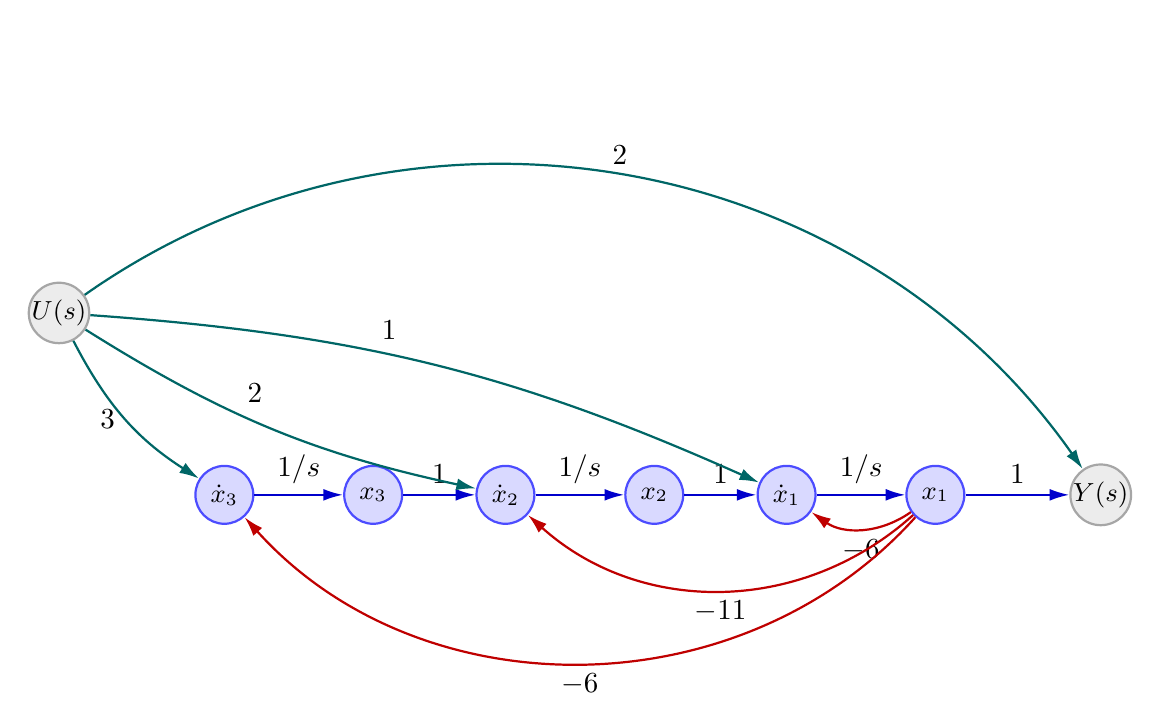
\begin{tikzpicture}[scale=1.05, transform shape]
    \node[sfgterminal] (U) at (0,2.2) {$U(s)$};
    \node[sfgnode] (dx3) at (2,0) {$\dot{x}_3$};
    \node[sfgnode] (x3) at (3.8,0) {$x_3$};
    \node[sfgnode] (dx2) at (5.4,0) {$\dot{x}_2$};
    \node[sfgnode] (x2) at (7.2,0) {$x_2$};
    \node[sfgnode] (dx1) at (8.8,0) {$\dot{x}_1$};
    \node[sfgnode] (x1) at (10.6,0) {$x_1$};
    \node[sfgterminal] (Y) at (12.6,0) {$Y(s)$};
    
    % Integrators
    \draw[sfgarrow] (dx3) -- node[above] {$1/s$} (x3);
    \draw[sfgarrow] (x3) -- node[above] {$1$} (dx2);
    \draw[sfgarrow] (dx2) -- node[above] {$1/s$} (x2);
    \draw[sfgarrow] (x2) -- node[above] {$1$} (dx1);
    \draw[sfgarrow] (dx1) -- node[above] {$1/s$} (x1);
    \draw[sfgarrow] (x1) -- node[above] {$1$} (Y);
    
    % Inputs
    \draw[sfgbypass] (U) to[bend right=15] node[left] {$3$} (dx3);
    \draw[sfgbypass] (U) to[bend right=10] node[pos=0.4, above right] {$2$} (dx2);
    \draw[sfgbypass] (U) to[bend left=10] node[pos=0.4, above right] {$1$} (dx1);
    \draw[sfgbypass] (U) to[bend left=45] node[above] {$2$} (Y);
    
    % Feedbacks from x1
    \draw[sfgloop] (x1) to[bend left=35] node[below] {$-6$} (dx1);
    \draw[sfgloop] (x1) to[bend left=42] node[below] {$-11$} (dx2);
    \draw[sfgloop] (x1) to[bend left=48] node[below] {$-6$} (dx3);
\end{tikzpicture}
\end{center}

\textbf{(b) Analisis Dualitas Transpos}

Dengan membandingkan hasil pada Soal 9 (CCF) dan Soal 10 (OCF):
$$A_{OCF} = \begin{bmatrix} -6 & 1 & 0 \\ -11 & 0 & 1 \\ -6 & 0 & 0 \end{bmatrix} \quad \longleftrightarrow \quad A_{CCF}^T = \begin{bmatrix} 0 & 0 & -6 \\ 1 & 0 & -11 \\ 0 & 1 & -6 \end{bmatrix}$$
Melalui pembalikan urutan indeks koordinat variabel keadaan ($x_i \leftrightarrow x_{n+1-i}$), terlihat bahwa:
$$A_{OCF} \sim A_{CCF}^T, \quad B_{OCF} \sim C_{CCF}^T, \quad C_{OCF} \sim B_{CCF}^T, \quad D_{OCF} = D_{CCF}$$
Hal ini membuktikan sifat dualitas formal antara keterkontrolan dan keterobservasian dalam representasi kanonik ruang keadaan.

\vspace{12pt}
\hrule
\vspace{10pt}

% =========================================================================
% SOAL 11
% =========================================================================
\textbf{\large No. 11}

\textbf{Soal:}  
Diberikan fungsi alih sistem:
$$G(s) = \frac{s + 3}{(s + 1)(s + 2)(s + 4)}$$
Bentuklah representasi ruang keadaan dalam Bentuk Kanonik Kaskade (\textit{Cascade/Series Form}) melalui faktorisasi menjadi perkalian tiga subsistem orde pertama berurutan $G(s) = G_1(s) G_2(s) G_3(s) = \left(\frac{1}{s+1}\right)\left(\frac{s+3}{s+2}\right)\left(\frac{1}{s+4}\right)$ dan gambarkan diagram alirannya.

\textbf{Penyelesaian:}

Didefinisikan sinyal perantara pada setiap tahapan kaskade:

Subsistem pertama:
$$X_1(s) = \frac{1}{s+1} U(s) \implies \dot{x}_1(t) = -x_1(t) + u(t)$$

Subsistem kedua: Masukan subsistem adalah $x_1(t)$ dan keluarannya adalah $v(t)$:
$$V(s) = \frac{s+3}{s+2} X_1(s) = \left( 1 + \frac{1}{s+2} \right) X_1(s)$$
Didefinisikan variabel keadaan kedua $X_2(s) = \frac{1}{s+2} X_1(s) \implies \dot{x}_2(t) = -2 x_2(t) + x_1(t)$, sehingga $v(t) = x_2(t) + x_1(t)$.

Subsistem ketiga: Masukan subsistem adalah $v(t)$ dan keluarannya adalah $y(t)$:
$$Y(s) = \frac{1}{s+4} V(s) = \frac{1}{s+4} [X_2(s) + X_1(s)]$$
Dengan mendefinisikan variabel keadaan ketiga $x_3(t) = y(t)$, diperoleh:
$$\dot{x}_3(t) = -4 x_3(t) + x_1(t) + x_2(t)$$

Penggabungan seluruh persamaan dinamika menghasilkan sistem ruang keadaan berstruktur segitiga bawah (\textit{lower triangular}):
$$\begin{bmatrix} \dot{x}_1 \\ \dot{x}_2 \\ \dot{x}_3 \end{bmatrix} = \begin{bmatrix} -1 & 0 & 0 \\ 1 & -2 & 0 \\ 1 & 1 & -4 \end{bmatrix} \begin{bmatrix} x_1 \\ x_2 \\ x_3 \end{bmatrix} + \begin{bmatrix} 1 \\ 0 \\ 0 \end{bmatrix} u(t)$$
Persamaan keluaran adalah:
$$y(t) = \begin{bmatrix} 0 & 0 & 1 \end{bmatrix} \begin{bmatrix} x_1 \\ x_2 \\ x_3 \end{bmatrix} + [0] u(t)$$

\begin{center}
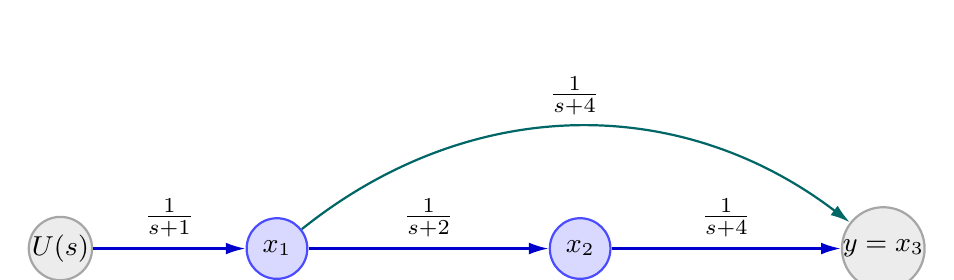
\begin{tikzpicture}[scale=1.1, transform shape]
    \node[sfgterminal] (U) at (0,0) {$U(s)$};
    \node[sfgnode] (x1) at (2.5,0) {$x_1$};
    \node[sfgnode] (x2) at (6,0) {$x_2$};
    \node[sfgterminal] (x3) at (9.5,0) {$y = x_3$};
    
    % Integrators/blocks
    \draw[sfgarrow] (U) -- node[above] {$\frac{1}{s+1}$} (x1);
    \draw[sfgarrow] (x1) -- node[above] {$\frac{1}{s+2}$} (x2);
    \draw[sfgarrow] (x2) -- node[above] {$\frac{1}{s+4}$} (x3);
    
    % Direct feedforward within cascade
    \draw[sfgbypass] (x1) to[bend left=38] node[above] {$\frac{1}{s+4}$} (x3);
\end{tikzpicture}
\end{center}

\vspace{12pt}
\hrule
\vspace{10pt}

% =========================================================================
% SOAL 12
% =========================================================================
\textbf{\large No. 12}

\textbf{Soal:}  
Diberikan fungsi alih yang memiliki kombinasi pole real sederhana dan pole kompleks konjugat:
$$G(s) = \frac{5s^2 + 17s + 18}{(s + 1)(s^2 + 4s + 5)}$$
\begin{enumerate}[label=(\alph*)]
    \item Lakukan ekspansi pecahan parsial dari fungsi alih tersebut.
    \item Susun representasi ruang keadaan dalam Bentuk Kanonik Modal Real (\textit{Real Modal / Diagonal Form}).
\end{enumerate}

\textbf{Penyelesaian:}

\textbf{(a) Ekspansi Pecahan Parsial}

Faktor penyebut kuadratik memiliki akar-akar kompleks $s = -2 \pm j$. Fungsi alih diekspansikan ke dalam bentuk:
$$G(s) = \frac{c_1}{s + 1} + \frac{\alpha s + \beta}{s^2 + 4s + 5}$$

Koefisien $c_1$ dihitung dengan metode penutupan Heaviside:
$$c_1 = \lim_{s \to -1} (s+1) G(s) = \frac{5(-1)^2 + 17(-1) + 18}{(-1)^2 + 4(-1) + 5} = \frac{5 - 17 + 18}{1 - 4 + 5} = \frac{6}{2} = 3$$

Pengurangan suku pecahan pertama dari fungsi alih total menghasilkan bagian kedua:
\begin{align*}
    \frac{\alpha s + \beta}{s^2 + 4s + 5} &= \frac{5s^2 + 17s + 18 - 3(s^2 + 4s + 5)}{(s+1)(s^2 + 4s + 5)} \\
    &= \frac{2s^2 + 5s + 3}{(s+1)(s^2 + 4s + 5)} = \frac{(s+1)(2s + 3)}{(s+1)(s^2 + 4s + 5)} = \frac{2s + 3}{s^2 + 4s + 5}
\end{align*}

Sehingga ekspansi pecahan parsial lengkapnya adalah:
$$G(s) = \frac{3}{s+1} + \frac{2s + 3}{s^2 + 4s + 5}$$

\textbf{(b) Formulasi Bentuk Kanonik Modal Real}

Untuk suku pole real $s = -1$, didefinisikan variabel keadaan $\dot{x}_1 = -x_1 + u$ dengan kontribusi keluaran $y_1 = 3 x_1$.
Untuk bagian kompleks kuadratik $\frac{2s+3}{s^2+4s+5}$, digunakan representasi ruang keadaan modal $2\times 2$ dengan pole $-\sigma \pm j\omega_d = -2 \pm j1$:
$$\begin{bmatrix} \dot{x}_2 \\ \dot{x}_3 \end{bmatrix} = \begin{bmatrix} -2 & 1 \\ -1 & -2 \end{bmatrix} \begin{bmatrix} x_2 \\ x_3 \end{bmatrix} + \begin{bmatrix} 2 \\ -1 \end{bmatrix} u(t)$$

Dengan menggabungkan seluruh moda, matriks ruang keadaan modal real sistem adalah:
$$A = \begin{bmatrix} -1 & 0 & 0 \\ 0 & -2 & 1 \\ 0 & -1 & -2 \end{bmatrix}, \quad B = \begin{bmatrix} 1 \\ 2 \\ -1 \end{bmatrix}, \quad C = \begin{bmatrix} 3 & 1 & 0 \end{bmatrix}, \quad D = [0]$$

\vspace{12pt}
\hrule
\vspace{10pt}

% =========================================================================
% SOAL 13
% =========================================================================
\textbf{\large No. 13}

\textbf{Soal:}  
Diberikan fungsi alih yang memiliki pole berulang berorde 3:
$$G(s) = \frac{3s^2 + 14s + 19}{(s + 2)^3}$$
\begin{enumerate}[label=(\alph*)]
    \item Lakukan ekspansi pecahan parsial dari fungsi alih tersebut.
    \item Tentukan representasi ruang keadaan dalam Bentuk Kanonik Jordan (\textit{Jordan Canonical Form}).
\end{enumerate}

\textbf{Penyelesaian:}

\textbf{(a) Ekspansi Pecahan Parsial Suku Pole Berulang}

Bentuk umum ekspansi pecahan parsial untuk pole berulang orde-3 adalah:
$$G(s) = \frac{c_1}{s + 2} + \frac{c_2}{(s + 2)^2} + \frac{c_3}{(s + 2)^3}$$

Dengan melakukan subtitusi variabel $p = s + 2 \implies s = p - 2$:
$$3s^2 + 14s + 19 = 3(p-2)^2 + 14(p-2) + 19 = 3(p^2 - 4p + 4) + 14p - 28 + 19 = 3p^2 + 2p + 3$$

Dengan membagi setiap suku oleh $p^3 = (s+2)^3$, diperoleh:
$$G(s) = \frac{3p^2 + 2p + 3}{p^3} = \frac{3}{p} + \frac{2}{p^2} + \frac{3}{p^3} = \frac{3}{s + 2} + \frac{2}{(s + 2)^2} + \frac{3}{(s + 2)^3}$$
Sehingga koefisien residu bertingkat adalah $c_1 = 3, c_2 = 2, c_3 = 3$.

\textbf{(b) Formulasi Bentuk Kanonik Jordan}

Didefinisikan variabel keadaan berantai (\textit{integrator chain with feedback $-2$}):
$$X_3(s) = \frac{1}{s+2} U(s) \implies \dot{x}_3(t) = -2 x_3(t) + u(t)$$
$$X_2(s) = \frac{1}{s+2} X_3(s) \implies \dot{x}_2(t) = -2 x_2(t) + x_3(t)$$
$$X_1(s) = \frac{1}{s+2} X_2(s) \implies \dot{x}_1(t) = -2 x_1(t) + x_2(t)$$

Keluaran sistem merupakan kombinasi linear dari ketiga variabel keadaan:
$$Y(s) = 3 X_3(s) + 2 X_2(s) + 3 X_1(s) \implies y(t) = 3 x_1(t) + 2 x_2(t) + 3 x_3(t)$$

Dalam representasi matriks, matriks dinamik $A$ memiliki blok Jordan berukuran $3 \times 3$ dengan superdiagonal bernilai 1:
$$A = \begin{bmatrix} -2 & 1 & 0 \\ 0 & -2 & 1 \\ 0 & 0 & -2 \end{bmatrix}, \quad B = \begin{bmatrix} 0 \\ 0 \\ 1 \end{bmatrix}, \quad C = \begin{bmatrix} 3 & 2 & 3 \end{bmatrix}, \quad D = [0]$$

\begin{center}
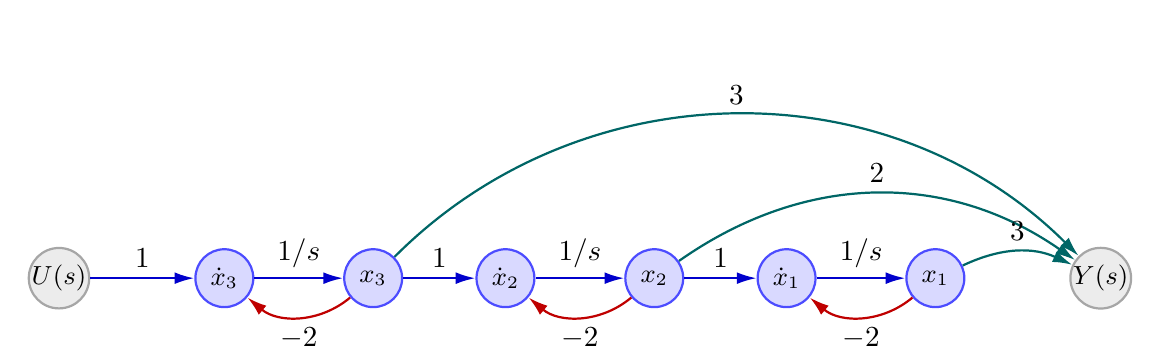
\begin{tikzpicture}[scale=1.05, transform shape]
    \node[sfgterminal] (U) at (0,0) {$U(s)$};
    \node[sfgnode] (dx3) at (2,0) {$\dot{x}_3$};
    \node[sfgnode] (x3) at (3.8,0) {$x_3$};
    \node[sfgnode] (dx2) at (5.4,0) {$\dot{x}_2$};
    \node[sfgnode] (x2) at (7.2,0) {$x_2$};
    \node[sfgnode] (dx1) at (8.8,0) {$\dot{x}_1$};
    \node[sfgnode] (x1) at (10.6,0) {$x_1$};
    \node[sfgterminal] (Y) at (12.6,0) {$Y(s)$};
    
    % Forward integrator chain
    \draw[sfgarrow] (U) -- node[above] {$1$} (dx3);
    \draw[sfgarrow] (dx3) -- node[above] {$1/s$} (x3);
    \draw[sfgarrow] (x3) -- node[above] {$1$} (dx2);
    \draw[sfgarrow] (dx2) -- node[above] {$1/s$} (x2);
    \draw[sfgarrow] (x2) -- node[above] {$1$} (dx1);
    \draw[sfgarrow] (dx1) -- node[above] {$1/s$} (x1);
    
    % Local feedbacks of eigenvalue -2
    \draw[sfgloop] (x3) to[bend left=40] node[below] {$-2$} (dx3);
    \draw[sfgloop] (x2) to[bend left=40] node[below] {$-2$} (dx2);
    \draw[sfgloop] (x1) to[bend left=40] node[below] {$-2$} (dx1);
    
    % Output taps
    \draw[sfgbypass] (x3) to[bend left=45] node[above] {$3$} (Y);
    \draw[sfgbypass] (x2) to[bend left=35] node[above] {$2$} (Y);
    \draw[sfgbypass] (x1) to[bend left=25] node[above] {$3$} (Y);
\end{tikzpicture}
\end{center}

\vspace{12pt}
\hrule
\vspace{10pt}

% =========================================================================
% SOAL 14
% =========================================================================
\textbf{\large No. 14}

\textbf{Soal:}  
Tentukan realisasi ruang keadaan matriks $(A, B, C, D)$ untuk sistem multivariabel berikut:
\begin{enumerate}[label=(\alph*)]
    \item Sistem Satu Masukan Dua Keluaran (SIMO):
    $$\mathbf{G}_{SIMO}(s) = \begin{bmatrix} \frac{s + 1}{s^2 + 5s + 6} \\ \frac{2s + 3}{s^2 + 5s + 6} \end{bmatrix}$$
    \item Sistem Dua Masukan Satu Keluaran (MISO):
    $$\mathbf{G}_{MISO}(s) = \begin{bmatrix} \frac{s + 4}{s^2 + 3s + 2} & \frac{2s + 1}{s^2 + 3s + 2} \end{bmatrix}$$
\end{enumerate}

\textbf{Penyelesaian:}

\textbf{(a) Realisasi SIMO ke Bentuk Controllable Canonical Form}

Kedua kanal keluaran memiliki penyebut karakteristik bersama $d(s) = s^2 + 5s + 6$ dengan $a_1 = 5, a_0 = 6$.
Pembilang keluaran pertama adalah $n_1(s) = s + 1 \implies b_{1,1} = 1, b_{1,0} = 1$.
Pembilang keluaran kedua adalah $n_2(s) = 2s + 3 \implies b_{2,1} = 2, b_{2,0} = 3$.

Matriks $A$ dan vektor masukan $B$ dibangun dari penyebut bersama:
$$A = \begin{bmatrix} 0 & 1 \\ -a_0 & -a_1 \end{bmatrix} = \begin{bmatrix} 0 & 1 \\ -6 & -5 \end{bmatrix}, \quad B = \begin{bmatrix} 0 \\ 1 \end{bmatrix}$$

Matriks keluaran $C$ berukuran $2 \times 2$ dibentuk dari koefisien masing-masing pembilang:
$$C = \begin{bmatrix} b_{1,0} & b_{1,1} \\ b_{2,0} & b_{2,1} \end{bmatrix} = \begin{bmatrix} 1 & 1 \\ 3 & 2 \end{bmatrix}, \quad D = \begin{bmatrix} 0 \\ 0 \end{bmatrix}$$

\textbf{(b) Realisasi MISO ke Bentuk Observable Canonical Form}

Penyebut bersama adalah $d(s) = s^2 + 3s + 2$ dengan $a_1 = 3, a_0 = 2$.
Pembilang masukan pertama adalah $n_1(s) = s + 4 \implies b_{1,1} = 1, b_{1,0} = 4$.
Pembilang masukan kedua adalah $n_2(s) = 2s + 1 \implies b_{2,1} = 2, b_{2,0} = 1$.

Matriks $A$ dan vektor keluaran $C$ dibangun dalam bentuk kanonik terobservasi:
$$A = \begin{bmatrix} -a_1 & 1 \\ -a_0 & 0 \end{bmatrix} = \begin{bmatrix} -3 & 1 \\ -2 & 0 \end{bmatrix}, \quad C = \begin{bmatrix} 1 & 0 \end{bmatrix}$$

Matriks masukan $B$ berukuran $2 \times 2$ dibentuk dari koefisien masing-masing pembilang kanal masukan:
$$B = \begin{bmatrix} b_{1,1} & b_{2,1} \\ b_{1,0} & b_{2,0} \end{bmatrix} = \begin{bmatrix} 1 & 2 \\ 4 & 1 \end{bmatrix}, \quad D = \begin{bmatrix} 0 & 0 \end{bmatrix}$$

\vspace{12pt}
\hrule
\vspace{10pt}

% =========================================================================
% SOAL 15
% =========================================================================
\textbf{\large No. 15}

\textbf{Soal:}  
Diberikan matriks transfer multivariabel 2-masukan 2-keluaran (MIMO):
$$\mathbf{G}(s) = \begin{bmatrix} \frac{1}{s+1} & \frac{2}{s+2} \\ \frac{1}{(s+1)(s+2)} & \frac{1}{s+1} \end{bmatrix}$$
\begin{enumerate}[label=(\alph*)]
    \item Tentukan kutub-kutub karakteristik matriks alih dan lakukan ekspansi pecahan parsial matriks.
    \item Tentukan matriks residu $W_i$ untuk setiap kutub, hitung rank masing-masing matriks residu, dan lakukan dekomposisi dyadic rank $W_i = C_i B_i$.
    \item Susun matriks realisasi ruang keadaan minimal $(A, B, C, D)$ menggunakan Metode Gilbert dan verifikasi ordo minimalnya.
\end{enumerate}

\textbf{Penyelesaian:}

\textbf{(a) Ekspansi Pecahan Parsial Matriks Alih}

Penyebut sekutu terkecil dari seluruh entri matriks transfer adalah $(s+1)(s+2)$, sehingga kutub-kutub sistem adalah $s_1 = -1$ dan $s_2 = -2$. Matriks transfer diekspansikan ke dalam bentuk penjumlahan matriks residu:
$$\mathbf{G}(s) = \frac{W_1}{s + 1} + \frac{W_2}{s + 2}$$

\textbf{(b) Perhitungan Matriks Residu dan Dekomposisi Dyadic}

Matriks residu pertama pada kutub $s_1 = -1$:
$$W_1 = \lim_{s \to -1} (s+1) \mathbf{G}(s) = \lim_{s \to -1} \begin{bmatrix} 1 & \frac{2(s+1)}{s+2} \\ \frac{1}{s+2} & 1 \end{bmatrix} = \begin{bmatrix} 1 & 0 \\ 1 & 1 \end{bmatrix}$$
Determinan matriks residu pertama adalah $\det(W_1) = (1)(1) - (0)(1) = 1 \neq 0$, sehingga $\operatorname{rank}(W_1) = k_1 = 2$.
Karena ber-rank 2, dekomposisi dyadic dilakukan dengan memilih matriks identitas:
$$C_1 = W_1 = \begin{bmatrix} 1 & 0 \\ 1 & 1 \end{bmatrix}, \quad B_1 = I_2 = \begin{bmatrix} 1 & 0 \\ 0 & 1 \end{bmatrix}$$

Matriks residu kedua pada kutub $s_2 = -2$:
$$W_2 = \lim_{s \to -2} (s+2) \mathbf{G}(s) = \lim_{s \to -2} \begin{bmatrix} \frac{s+2}{s+1} & 2 \\ \frac{1}{s+1} & \frac{s+2}{s+1} \end{bmatrix} = \begin{bmatrix} 0 & 2 \\ -1 & 0 \end{bmatrix}$$
Determinan matriks residu kedua adalah $\det(W_2) = (0)(0) - (2)(-1) = 2 \neq 0$, sehingga $\operatorname{rank}(W_2) = k_2 = 2$.
Dekomposisi dyadic untuk residu kedua:
$$C_2 = W_2 = \begin{bmatrix} 0 & 2 \\ -1 & 0 \end{bmatrix}, \quad B_2 = I_2 = \begin{bmatrix} 1 & 0 \\ 0 & 1 \end{bmatrix}$$

\textbf{(c) Konstruksi Realisasi Minimal Gilbert}

Orde minimal sistem ruang keadaan adalah jumlah rank dari seluruh matriks residu:
$$n = k_1 + k_2 = 2 + 2 = 4$$

Matriks-matriks realisasi ruang keadaan dibentuk sebagai:
$$A = \begin{bmatrix} s_1 I_{k_1} & 0 \\ 0 & s_2 I_{k_2} \end{bmatrix} = \begin{bmatrix} -1 & 0 & 0 & 0 \\ 0 & -1 & 0 & 0 \\ 0 & 0 & -2 & 0 \\ 0 & 0 & 0 & -2 \end{bmatrix}$$
$$B = \begin{bmatrix} B_1 \\ B_2 \end{bmatrix} = \begin{bmatrix} 1 & 0 \\ 0 & 1 \\ 1 & 0 \\ 0 & 1 \end{bmatrix}$$
$$C = \begin{bmatrix} C_1 & C_2 \end{bmatrix} = \begin{bmatrix} 1 & 0 & 0 & 2 \\ 1 & 1 & -1 & 0 \end{bmatrix}$$
$$D = \lim_{s \to \infty} \mathbf{G}(s) = \begin{bmatrix} 0 & 0 \\ 0 & 0 \end{bmatrix}$$

Karena seluruh baris $B$ dan kolom $C$ tidak ada yang nol serta rank keterkontrolan dan keterobservasian penuh ($n = 4$), realisasi $(A, B, C, D)$ di atas terbukti merupakan realisasi ruang keadaan minimal berorde 4 bagi matriks transfer $\mathbf{G}(s)$.

\end{document}
